% slides.tex — Lund University inspired title slide + content slide mock
\documentclass[aspectratio=169]{beamer}

% keep presentation lightweight and self-contained
\usetheme{default}
\setbeamertemplate{navigation symbols}{}
\setbeamertemplate{headline}{}

\usepackage{tikz}
\usetikzlibrary{calc}
\usepackage{graphicx}
\usepackage{ragged2e}
\usepackage{calc}
\usepackage{xcolor}
\usepackage{iftex}

\ifPDFTeX
  \usepackage[T1]{fontenc}
  \usepackage[utf8]{inputenc}
  \usepackage{mathptmx} % Times-like serif
  \usepackage[scaled=0.92]{helvet} % Arial-like sans
  \newcommand{\TitleFont}{\rmfamily}
  \newcommand{\SubtitleFont}{\sffamily}
\else
  \usepackage{fontspec}
  \setmainfont{Times New Roman}
  \newfontfamily\TitleFont{Times New Roman}[Scale=1.0]
  \newfontfamily\SubtitleFont{Arial}[Scale=1.0]
\fi

% --- Color palette sampled from Presentation-template-page1.jpg ---
\definecolor{LUBeige}{HTML}{D8CCAA}
\definecolor{LUBronze}{HTML}{8A4F16}

% ensure other frames revert to a neutral background
\setbeamercolor{background canvas}{bg=white}
\setbeamercolor{normal text}{fg=black}
\setbeamercolor{footline}{fg=LUBronze,bg=white!0}


\newdimen\CircleRadius
\CircleRadius=0.46\paperheight
\newlength{\ContentHeight} % matched to left-column content height on content slides
\newlength{\ImageHeight}
\newlength{\ImageWidth}
\newlength{\ImageInnerHeight}
\newlength{\ImageInnerWidth}

\title{Module 5: Ethical aspects of AI-aided content analysis}
\subtitle{Lesson 5.1: Key takeaways and ethical perspectives \\[0.8em]nils.holmberg@iko.lu.se}
\author{}

% Custom footline with frame number (left) and compact logo (right)
\setbeamertemplate{footline}{%
  \vspace{0.35cm}% raises the footer slightly above the slide edge
  \begin{beamercolorbox}[wd=\paperwidth,ht=3ex,dp=1.2ex,leftskip=0.9cm,rightskip=0.9cm]{footline}
    {\SubtitleFont\small\color{LUBronze}\insertframenumber}
    \hfill
    \raisebox{-0.1cm}{
\includegraphics[height=0.75cm]{edulab-lulogo.png}}
  \end{beamercolorbox}%
}

% Bronze round bullets with matching text color for itemize blocks
\setbeamercolor{itemize item}{fg=LUBronze}
\setbeamercolor{itemize body}{fg=LUBronze}
\setbeamertemplate{itemize item}{\color{LUBronze}\scriptsize\raise0.2ex\hbox{\textbullet}}

\makeatletter
\defbeamertemplate*{title page}{lu}{%
  \begin{tikzpicture}[remember picture,overlay]
    % full-bleed beige background — adjust offsets here if you need more/less margin.
    \fill[LUBeige] (current page.south west) rectangle (current page.north east);

    % Lund University logo in the upper-left — tweak the shifts to nudge placement.
    \node[anchor=north west] at ([xshift=0.3cm,yshift=-0.25cm]current page.north west) {
      
\includegraphics[height=1.9cm]{edulab-lulogo.png}
    };

    % Circular pelican artwork, bottom cropped by slide edge — adjust center/radius as needed.
    \coordinate (circlecenter) at ([xshift=0.36\paperwidth,yshift=0.22\paperheight]current page.south west);
    \begin{scope}
      \clip (circlecenter) circle (\CircleRadius);
      \node at (circlecenter) {
        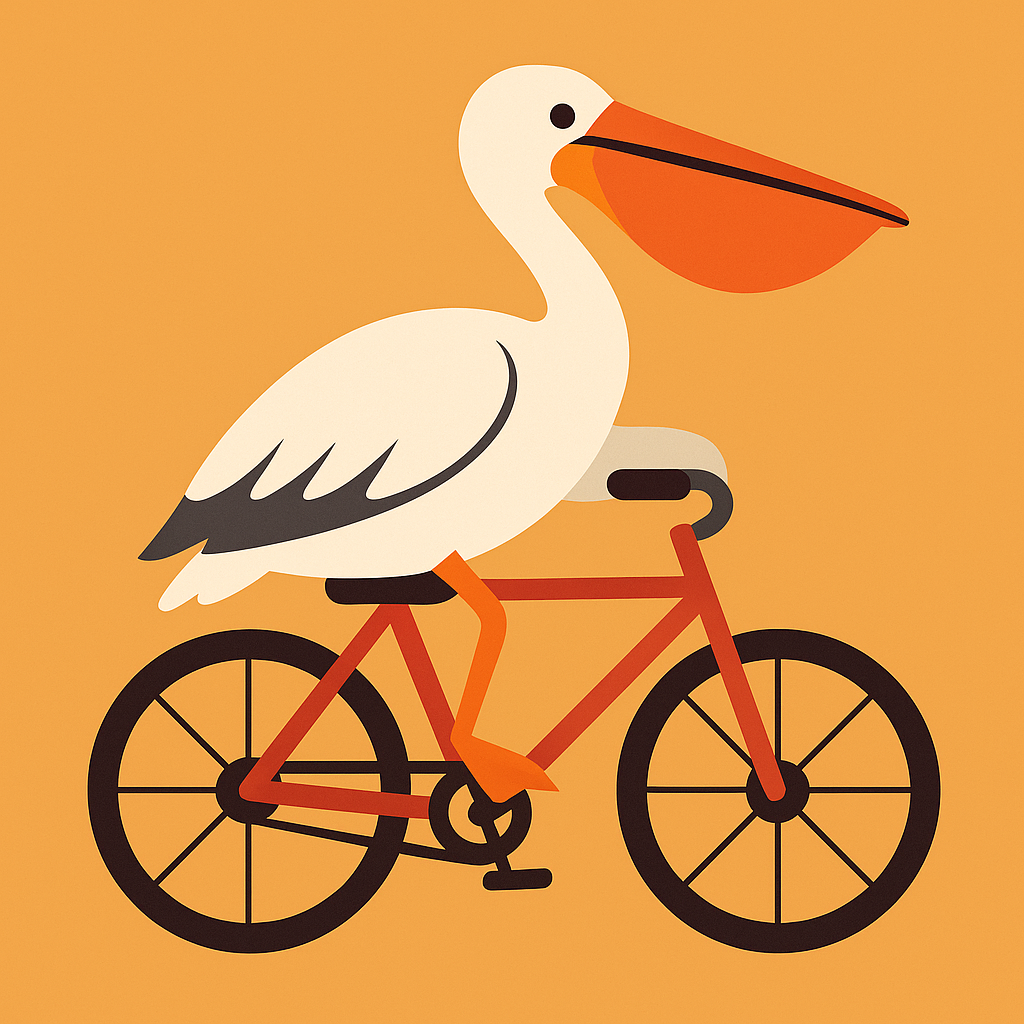
\includegraphics[width=1.12\paperheight]{pelican.png}
      };
    \end{scope}

    % Title block positioned on the right — tweak node shift/inner sep to fine-tune spacing.
    \node[anchor=north east] at ([xshift=-1.0cm,yshift=-1.0cm]current page.north east) {
      \begin{tikzpicture}
        \node[anchor=north east, fill=white, inner sep=18pt, minimum width=0.48\paperwidth] (titlebox) at (0,0) {
          \begin{minipage}{0.44\paperwidth}
            \raggedright
            {\TitleFont\fontsize{14}{16}\selectfont\bfseries\color{LUBronze}\inserttitle\par}
            \vspace{0.5em}
            {\color{LUBronze}\rule{\linewidth}{0.8pt}\par}
            \vspace{0.4em}
            {\SubtitleFont\fontsize{11}{13}\selectfont\color{LUBronze}\insertsubtitle\par}
          \end{minipage}
        };
      \end{tikzpicture}
    };
  \end{tikzpicture}
}
\setbeamertemplate{title page}[lu]
\makeatother

\begin{document}

\setbeamercolor{background canvas}{bg=LUBeige}
\begin{frame}[plain]
  \titlepage
\end{frame}
\setbeamercolor{background canvas}{bg=white}
\setcounter{framenumber}{0} % so the first content slide starts at 1

\begin{frame}[t]{}
  \vspace*{0.5cm}
  {\TitleFont\fontsize{18}{22}\selectfont\color{LUBronze}Key takeaways and ethical perspectives\par}
  \vspace{0.3em}
  {\color{LUBronze}\rule{\linewidth}{0.8pt}}\par
  \vspace{0.2cm}
  \begin{columns}[t]
    \begin{column}[t]{0.4\textwidth}
      \vspace*{0pt}
      \begin{itemize}\setlength\itemsep{0.65em}
        \item AI for sustainability insights
        \item Low-code text and visuals
        \item Interpret machine learning findings
        \item Automation ethics boundaries
        \item Bias transparency accountability
      \end{itemize}
    \end{column}
    \begin{column}[t]{0.5\textwidth}
      \vspace*{0pt}
      
\includegraphics[
        width=\linewidth,
        height=0.60\textheight,
        keepaspectratio=false,
        trim=0 0 0 0,
        clip
      ]{5-1-1-video-lecture-slides-3.png}
    \end{column}
  \end{columns}
\end{frame}

\begin{frame}[t]{}
  \vspace*{0.5cm}
  {\TitleFont\fontsize{18}{22}\selectfont\color{LUBronze}What You Learned in This Course\par}
  \vspace{0.3em}
  {\color{LUBronze}\rule{\linewidth}{0.8pt}}\par
  \vspace{0.2cm}
  \begin{columns}[t]
    \begin{column}[t]{0.4\textwidth}
      \vspace*{0pt}
      \begin{itemize}\setlength\itemsep{0.65em}
        \item Collect sustainability source data
        \item Analyze text and visuals
        \item Apply NLP, vision methods
        \item Visualize communication patterns
        \item Link methods to messaging
      \end{itemize}
    \end{column}
    \begin{column}[t]{0.5\textwidth}
      \vspace*{0pt}
      
\includegraphics[
        width=\linewidth,
        height=0.55\textheight,
        keepaspectratio=false,
        trim=0 0 0 0,
        clip
      ]{5-1-1-video-lecture-slides-3.png}
    \end{column}
  \end{columns}
\end{frame}

\begin{frame}[t]{}
  \vspace*{0.5cm}
  {\TitleFont\fontsize{18}{22}\selectfont\color{LUBronze}Ethics of Automating Content Interpretation\par}
  \vspace{0.3em}
  {\color{LUBronze}\rule{\linewidth}{0.8pt}}\par
  \vspace{0.2cm}
  \begin{columns}[t]
    \begin{column}[t]{0.4\textwidth}
      \vspace*{0pt}
      \begin{itemize}\setlength\itemsep{0.65em}
        \item Probe algorithmic bias impacts
        \item Assess interpretability limits
        \item Center researcher validation role
        \item Respect privacy and consent
        \item Embed ethics in design
      \end{itemize}
    \end{column}
    \begin{column}[t]{0.5\textwidth}
      \vspace*{0pt}
      
\includegraphics[
        width=\linewidth,
        height=0.55\textheight,
        keepaspectratio=false,
        trim=0 0 0 0,
        clip
      ]{5-1-1-video-lecture-slides-3.png}
    \end{column}
  \end{columns}
\end{frame}

\begin{frame}[t]{}
  \vspace*{0.5cm}
  {\TitleFont\fontsize{18}{22}\selectfont\color{LUBronze}Analysis documentation and open science (Jupyter)\par}
  \vspace{0.3em}
  {\color{LUBronze}\rule{\linewidth}{0.8pt}}\par
  \vspace{0.2cm}
  \begin{columns}[t]
    \begin{column}[t]{0.4\textwidth}
      \vspace*{0pt}
      \begin{itemize}\setlength\itemsep{0.65em}
        \item Champion transparent workflows
        \item Share data code outputs
        \item Use cloud collaboration tools
        \item Enable peer replication
        \item Align practice with openness
%        \item Lab: download Colab notebook
      \end{itemize}
    \end{column}
    \begin{column}[t]{0.5\textwidth}
      \vspace*{0pt}
      
\includegraphics[
        width=\linewidth,
        height=0.55\textheight,
        keepaspectratio=false,
        trim=0 0 0 0,
        clip
      ]{5-1-1-video-lecture-slides-5.png}
    \end{column}
  \end{columns}
\end{frame}

\begin{frame}[t]{}
  \vspace*{0.5cm}
  {\TitleFont\fontsize{18}{22}\selectfont\color{LUBronze}Using Jupyter Notebooks to Ensure Reproducibility\par}
  \vspace{0.3em}
  {\color{LUBronze}\rule{\linewidth}{0.8pt}}\par
  \vspace{0.2cm}
  \begin{columns}[t]
    \begin{column}[t]{0.4\textwidth}
      \vspace*{0pt}
      \begin{itemize}\setlength\itemsep{0.65em}
        \item Quarto unifies code narratives
        \item Automate reproducible execution
        \item Convert easily across formats
        \item Embed metadata and settings
        \item Share transparent reports
      \end{itemize}
    \end{column}
    \begin{column}[t]{0.5\textwidth}
      \vspace*{0pt}
      
\includegraphics[
        width=\linewidth,
        height=0.55\textheight,
        keepaspectratio=false,
        trim=0 0 0 0,
        clip
      ]{5-1-1-video-lecture-slides-5.png}
    \end{column}
  \end{columns}
\end{frame}

\begin{frame}[t]{}
  \vspace*{0.5cm}
  {\TitleFont\fontsize{18}{22}\selectfont\color{LUBronze}Communicating AI-aided content analysis (Quarto)\par}
  \vspace{0.3em}
  {\color{LUBronze}\rule{\linewidth}{0.8pt}}\par
  \vspace{0.2cm}
  \begin{columns}[t]
    \begin{column}[t]{0.4\textwidth}
      \vspace*{0pt}
      \begin{itemize}\setlength\itemsep{0.65em}
        \item Translate findings for audiences
        \item Visualize sustainability patterns
        \item Link effects to strategy
        \item Clarify methods for all
        \item Situate findings ethically
%        \item Lab: convert notebook Quarto
      \end{itemize}
    \end{column}
    \begin{column}[t]{0.5\textwidth}
      \vspace*{0pt}
      
\includegraphics[
        width=\linewidth,
        height=0.55\textheight,
        keepaspectratio=false,
        trim=0 0 0 0,
        clip
      ]{5-1-1-video-lecture-slides-7.png}
    \end{column}
  \end{columns}
\end{frame}

\begin{frame}[t]{}
  \vspace*{0.5cm}
  {\TitleFont\fontsize{18}{22}\selectfont\color{LUBronze}Turning Your Analysis into a Research Publication\par}
  \vspace{0.3em}
  {\color{LUBronze}\rule{\linewidth}{0.8pt}}\par
  \vspace{0.2cm}
  \begin{columns}[t]
    \begin{column}[t]{0.4\textwidth}
      \vspace*{0pt}
      \begin{itemize}\setlength\itemsep{0.65em}
        \item Begin with documented notebook
        \item Clarify question and methods
        \item Use structured visual supports
        \item Align with existing literature
        \item Target relevant digital journals
      \end{itemize}
    \end{column}
    \begin{column}[t]{0.5\textwidth}
      \vspace*{0pt}
      
\includegraphics[
        width=\linewidth,
        height=0.55\textheight,
        keepaspectratio=false,
        trim=0 0 0 0,
        clip
      ]{5-1-1-video-lecture-slides-7.png}
    \end{column}
  \end{columns}
\end{frame}

\end{document}

